\documentclass[10pt,a4paper]{article}

\usepackage[nonatbib,final]{nips_2017}

\usepackage[utf8]{inputenc} % allow utf-8 input
\usepackage[T1]{fontenc}    % use 8-bit T1 fonts
\usepackage{hyperref}       % hyperlinks
\usepackage{url}            % simple URL typesetting
\usepackage{booktabs}       % professional-quality tables
\usepackage{amsfonts}       % blackboard math symbols
\usepackage{nicefrac}       % compact symbols for 1/2, etc.
\usepackage{microtype}      % microtypography
\usepackage{color} % DH add

%
\usepackage{makeidx}  % allows for indexgeneration
\usepackage{amsmath,graphicx,dsfont,bm}
\usepackage{textcomp}

%% hyphenation
\hyphenation{histo-patho-logy}

\usepackage{todonotes}

\newcommand{\abbr}[2]{#1 (#2)}
\newcommand{\abbrpl}[2]{#1s (#2)}

%% used in the method section
\newcommand{\norm}{f}
\newcommand{\normaldist}{\mathcal{N}}
\newcommand{\templateX}{\mathcal X}
\newcommand{\expect}{\mathds E}
\newcommand{\tx}{\tilde{x}}
\newcommand{\feature}{\mathcal{F}}
\newcommand{\transformer}{\mathcal{T}}
\newcommand{\addgate}{\beta}
\newcommand{\mulgate}{\gamma}
\newcommand{\bx}{\bm{x}}
\newcommand{\std}{\text{std}}
\newcommand{\tX}{\tilde{X}}
\newcommand{\lxl}{\ensuremath{1 \times 1} }

\newcommand{\cX}{\mathcal{X}}
\newcommand{\tcX}{\mathcal{\tilde{X}}}

\newcommand{\zz}{\mathbf{z}}
\newcommand{\yy}{\mathbf{y}}
\newcommand{\xx}{\mathbf{x}}
\newcommand{\txx}{\mathbf{\tilde{x}}}
\newcommand{\R}{\mathds{R}}

\newcommand{\X}{\mathcal{X}}
\newcommand{\Y}{\mathcal{Y}}
\newcommand{\Z}{\mathcal{Z}}
\newcommand{\U}{\mathcal{U}}
\newcommand{\V}{\mathcal{V}}
\newcommand{\I}{\mathcal{I}}
\renewcommand{\P}{\mathds{P}}

\newcommand{\inst}[1]{${}^{#1}$}

\hypersetup{
    pdftitle={Optimal Session-to-Session Transport for BCI},
    pdfauthor={Schneider et al.},
    pdfsubject={Optimal Session-to-Session Transport for BCI},
    pdfkeywords={Brain-Computer Interface, Machine Learning, Neuroscience, Domain Adaptation}
}

%
\title{Optimal Session-to-Session Transport for BCI}

\author{
  Steffen~Schneider\\
  Technical University of Munich, Munich, Germany\\
  \texttt{steffen.schneider@tum.de}
}

\begin{document}
\maketitle

\begin{abstract}
    In this report, we present and discuss a pipeline to classifier error-related potentials (ErrPs) in electroencephalography (EEG) recordings during a cursor movement task.
    We compare several approaches for preprocessing, feature selection and classification.
    Maybe surprisingly, good performance is obtained even with simple feature selection methods apply directly to the time traces.
    We obtain an ACC of XX \%, F1-score \%, AUC \% using a final ensemble of a Random Forest and SVM classifier.
    \footnote{The code for the approach is accessible at \texttt{github.com/stes/bci}.}
\end{abstract}

\section{Introduction}

%%

\cite{Cuturi2013,Ehrlich2016,Flamary2016,Spuler2015,Chai2017,Bug2017,Martin2013,Lotte2014,Li,Pan,Courty,silvoni2011brain,millan2010combining,lebedev2006brain,Stober2015,Ioffe2015batch}

\section{Methods}

\subsection{Feature Selection}

To determine the relevance of different time points, the t-statistic between the two classes is computed.
From this, the channel and timesteps of highest significance, i.e., with lowest $p$-value, is selected.
\footnote{Already at this point, we shall note that the t-test is not designed to compare p-values.
This is why the p-values here are of no statistical meaning of interest and should be considered as a mean to perform feature selection.}

For the baseline method, the identified timepoints were directly used for the further analysis.

\begin{itemize}
    \item Peak-Picking
    \item Signal Averaging
    \item Spectogram analysis
\end{itemize}

\subsection{Classification}

For robust classification, an ensemble classifier is constructed in order to obtain a measure of uncertainty over the predictions.
Candidates for the ensemble are Random Forest Classifiers (RFOs) and Support Vector Machines (SVMs) with variable hyperparameters.

The models are evaluated

\begin{enumerate}
    \item
\end{enumerate}

For the final evaluation, a 10-fold cross validation is used.


\subsection{Visualization}

As labels are not available for the validation set, we offer a qualitative evaluation of the classifier performance.

\subsection{Domain Adaptation by Optimal Transport}
In this work, we adapt the notion of domain adaptation also given in the review by \cite{Pan}.
A domain is denoted as a tuple $(\X, \P_{\X})$ of a space $\X$ and a distribution $\P_{\X}$.
In our setting, we do not only deal with a single source and a single target domain, but rather with a set of domains $\{ \X^k \}_{k=1}^N$ which are part of a common signal space $\U \supset \X^k\ \forall k \in [N]$.
We consider each domain here to be fully defined as a set of samples directly given by $\X^k := \{\xx^{(j)}\}_{j=1}^{N_k}$ drawn \emph{i.i.d.} from $\P_{\X}$.

As a last requirement, we assume that a feature space $\V$ and \emph{measurement functions} $\Phi^k: \V \mapsto X^k$ exists such that for each $\xx \in \X^k$, there exists $v \in \V$ with $\Phi^k(v) = \xx^k$.
This view can also be extended in a probabilistic way by adding noise to the measurement process.
For a subset of domains with $k \in \I$, labels $\Y^k = \{y^{(j)}\}_{j=1}^{N_k}$ are available.
Goal of the adaptation is to be able to apply an algorithm fitted to $(\X^\I, \Y^\I)$ on all data domains by transforming $\xx \in \X^k$ to $\xx' \in \X^\I$ such that the latent representation $v \in \V$ (the content) of both samples is preserved.

Recently \cite{Courty} presented a methods to apply mechanisms from optimal transport \cite{Cuturi2013,Flamary2016} to this domain adaptation problem.
We evaluate Optimal Transport for session-to-session transfer in the detection of ErrPs.
The general scheme of transferring a source to the target domain using label information is depicted in figure~\ref{fig:optimal-transport}.

\begin{figure}
    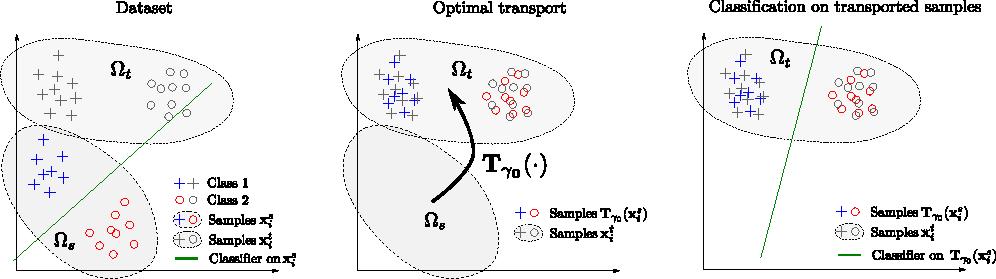
\includegraphics[width=\textwidth]{img/ot.pdf}
    \caption{Schematic overview of optimal transport. Given the source and target domains $\Omega_s$ and $\Omega_t$, optimal transport is used to compute a mapping $T$ between source and target domain, transforming the training dataset to match the target distribution.
    Finally, the classifier is fitted to $T(\Omega_s)$, making it more suitable for classifying the data from $\Omega_t$.
    In the context of BCI research, we propose the use of this technique between features from different sessions or subjects.
    Reproduced from \cite{Courty}.}
    \label{fig:optimal-transport}
\end{figure}

\section{Experiments}

Two datasets were considered for the evaluation procedure.
In addition to the original dataset, we evaluated classifier performance on the BCI dataset by \cite{TODO}.
We evaluate the approach on the ICS ERP Dataset, which is comprised of 300 training and 300 validation epochs.
However, in this report, we will only report results for the ICS ERP dataset.

\subsection{Feature Selection}

Results on the training set in figure~\ref{fig-overview}~A yield timepoints of 208.9~ms for the N200 and 291.1~ms for the P300 responses.
Especially during the P300 response, highest differences are observed in the Cz electrode.
During the N200 response and the later response denoted as P400 (which is probably a delated P300), we found the Pz electrode to offer the best discriminative power.

As one qualitative measure of test performance, we compute the same statistics for the test set and compare these timesteps.
While the N200 and P400 responses are very consistent over datasets, a significant shift could be observed for the exact P300 timepoints.

\begin{figure}
    Train\\
    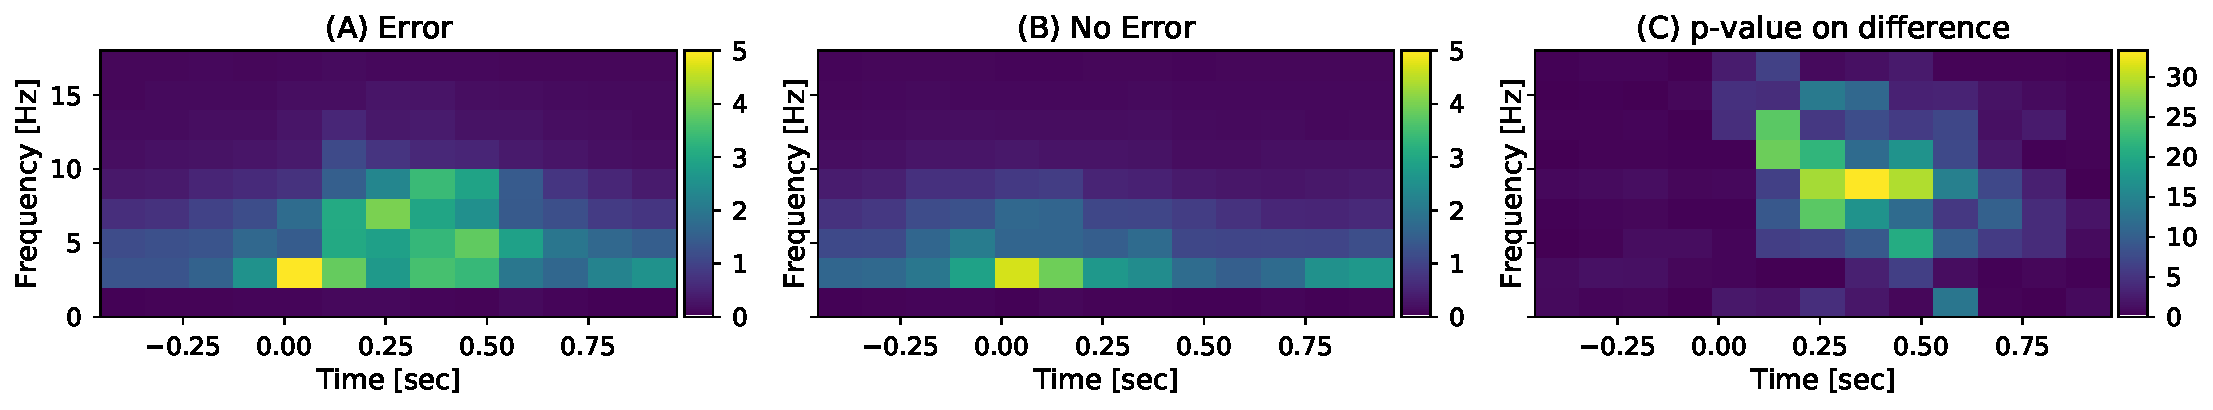
\includegraphics[width=\textwidth]{fig/spectrogram-train}
    Test\\
    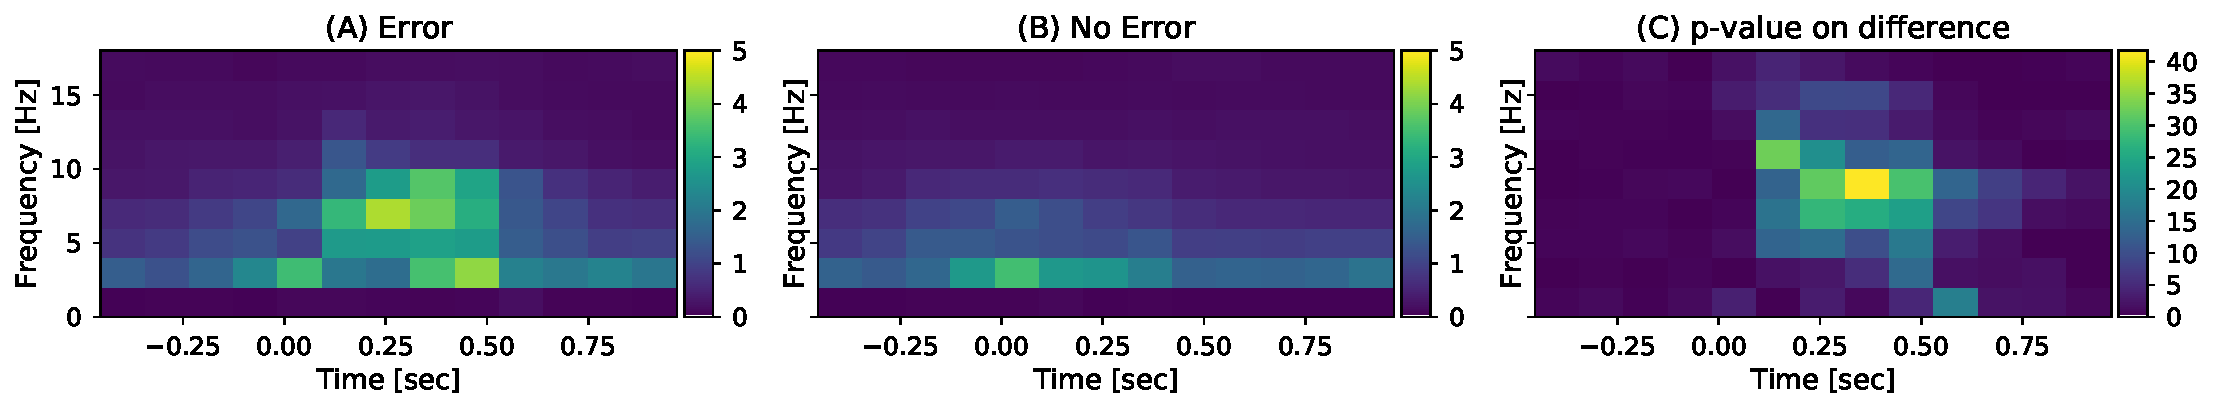
\includegraphics[width=\textwidth]{fig/spectrogram-test}
    \caption{Spectrogram analysis of the dataset. (A) and (B) depict the mean spectograms for the Cz channel during Error and NoError events, respectively. To evaluate discriminative power, a p-test is performed between the samples, yielding the distribution depicted in (C) for the Cz channel.}
\end{figure}

\begin{figure}
    (A) Training Set\\
    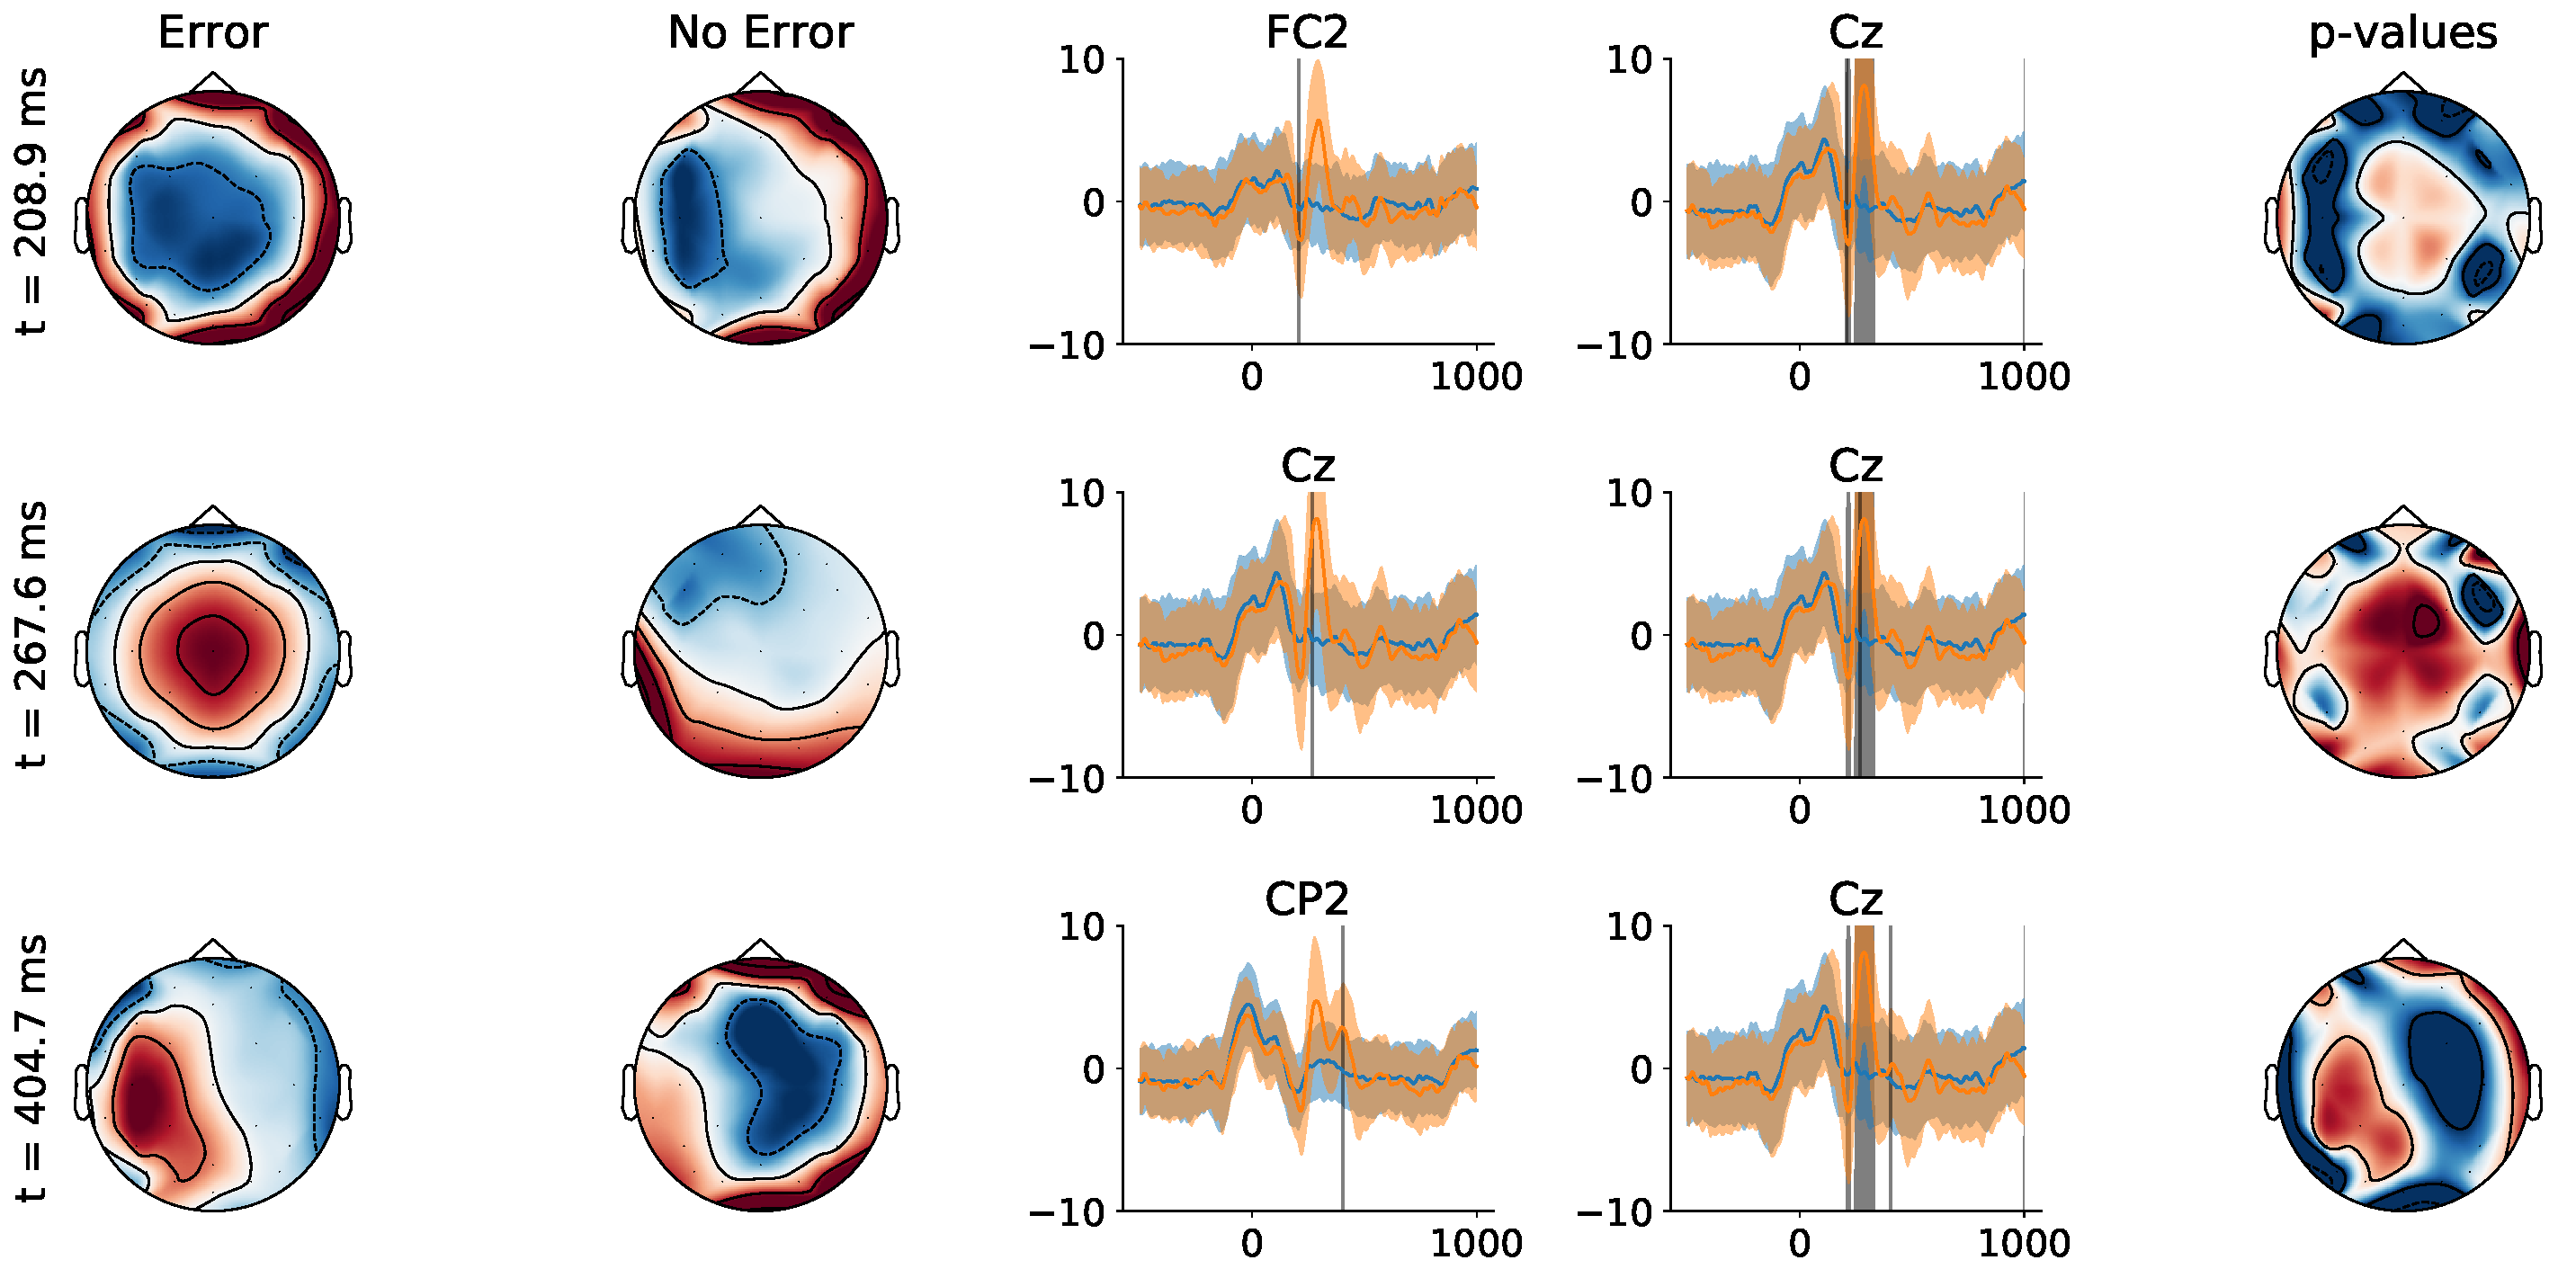
\includegraphics[width=\textwidth]{fig/overview-train}
    \vspace{12pt}\\
    (B) Test Set\\
    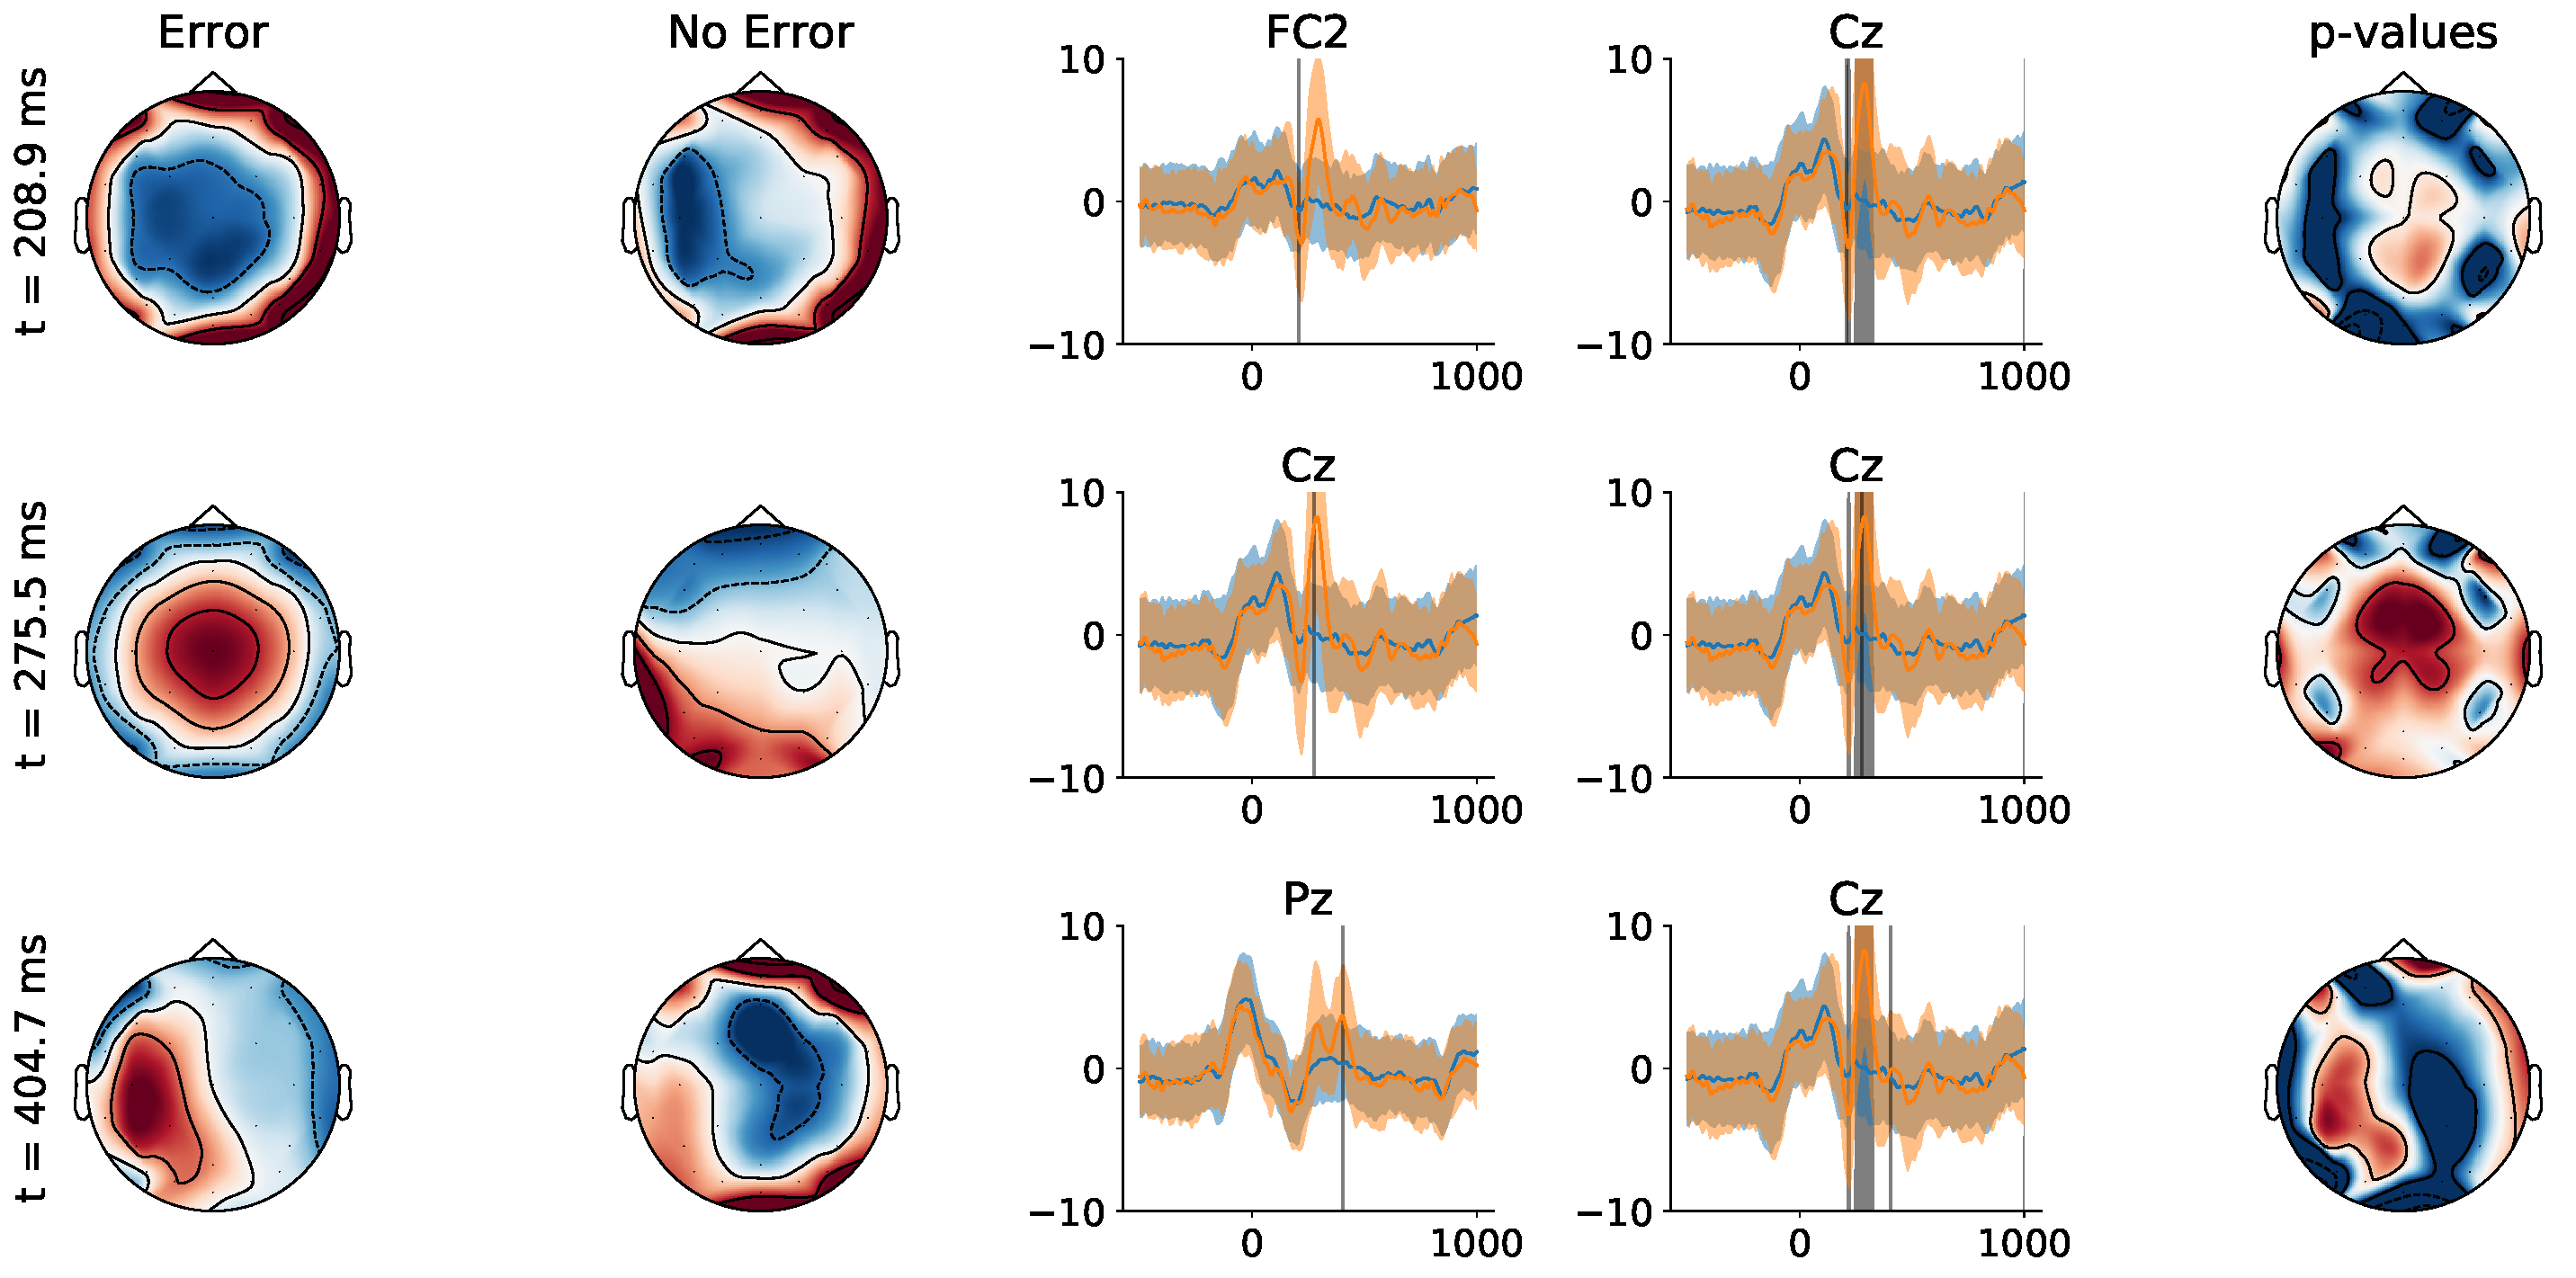
\includegraphics[width=\textwidth]{fig/overview-test}
    \caption{Spectrogram analysis of the test dataset. (A) and (B) depict the mean spectograms for the Cz channel during Error and NoError events, respectively. To evaluate discriminative power, a p-test is performed between the samples, yielding the distribution depicted in (C) for the Cz channel.}
\end{figure}

\subsection{Classifiers}

Given the limited amount of data samples, we evaluated the use of SVMs and Random Forests as the classifiers.
Data was preprocessed using an Independent Component Analysis (ICA).

We select most significant points for the different events:

\begin{itemize}
    \item N200: $[180\text{ms},210\text{ms}]$
    \item P300: $[250\text{ms},350\text{ms}]$
    \item delayed P300: $[350\text{ms},450\text{ms}]$
\end{itemize}

% Methods
Quite consistently, we found that linear SVMs outperform RFOs and RBF SVMS in classification performance.
Below, we report the cross-validation results for the approaches:

\begin{itemize}
    \item RFO: The number of tree ensembles was varied between 2 and 20.
    After cross-validation, the value was fixed to 18
    \item Linear SVM: The regularization parameter $C$ was varied from $10^{-6}$ to $10^2$.
    Best performance was obtained for $10^{-1} \dots 1.5$.
    \item RBF SVM: The regulariziation parameter was varied in the same range as for the linear SVM.
    However, no satisfying performance was obtained for the simple feature set, which is why this method
    was dismissed after cross validation
\end{itemize}

\begin{table}
\begin{tabular}{llll}
\toprule
{Fold} &    LDA & LinSVM & RFO\\
\midrule
0 & 87.2 \% &             85.7 \% &          85.7 \% \\
1 & 86.8 \% &             86.2 \% &          84.8 \% \\
2 & 88.3 \% &             88.3 \% &          88.0 \% \\
3 & 85.7 \% &             85.8 \% &          84.7 \% \\
4 & 87.5 \% &             87.8 \% &          85.7 \% \\
\bottomrule
\end{tabular}
\caption{Results}
\end{table}

\begin{table}
\begin{tabular}{lllll}
\toprule
{} & Ensemble &  Final & OT Ensemble & OT Final \\
\midrule
0 &   86.7 \% & 90.3 \% &     100.0 \% &  100.0 \% \\
1 &   89.0 \% & 90.0 \% &     100.0 \% &  100.0 \% \\
2 &   81.7 \% & 76.0 \% &     100.0 \% &   98.0 \% \\
3 &   85.7 \% & 81.0 \% &     100.0 \% &   98.7 \% \\
4 &   88.0 \% & 87.3 \% &     100.0 \% &   99.3 \% \\
5 &   89.7 \% & 92.3 \% &     100.0 \% &   98.7 \% \\
6 &   81.7 \% & 89.3 \% &     100.0 \% &  100.0 \% \\
7 &   91.0 \% & 91.7 \% &     100.0 \% &   99.3 \% \\
8 &   85.3 \% & 88.0 \% &     100.0 \% &  100.0 \% \\
9 &   95.7 \% & 97.0 \% &     100.0 \% &  100.0 \% \\
\bottomrule
\end{tabular}
\end{table}

\subsection{Session-to-session Transfer}
Using the Tübingen Dataset, we estimated performance in session-to-session transfer settings.

\section{Discussion}

Given the small size of the dataset, interpretation of performance and generalization of the results presented here should be done with care.


\paragraph{Adaptive Normalization Techniques}

We propose the use of techniques known from style transfer \cite{Gatys2016} to perform domain adaptation for medical data.
While the original algorithm was based on an iterative optimization algorithm, recent work deals with training a deep neural network to perform feed-forward stylization.
Interestingly, it was shown that it is sufficient to retrain the parameters of the network's Batch Normalization \cite{Ioffe2015} layers.
Inspired by this technique, Instance Normalization \cite{Ulyanov2016} and Adaptive Instance Normalization \cite{Huang2017} were developed.
In the context of color normalization for domain adaptation in digital pathology, Feature Aware Normalization (FAN) \cite{Bug2017} was developed using similar underlying principles.

Building on the work of \cite{Bug2017}, we investigate FAN for artifact removal and normalization of EEG signals and other electrophysiological recordings.
For training, the domains $\X^k$ can be chosen to match patients (subject-to-subject transfer), time (session-to-session transfer) or the signal acquisition equipment.

\footnotesize
\bibliographystyle{abbrv}
\bibliography{ref}

\newpage
\begin{appendix}

    \section{Analysis}

\end{appendix}

\end{document}
